\begin{activity}\label{A:0.3.2}
    \ba
        \item Based on symmetry alone, is $f(x) = x^2$ an even or an odd function?
        \item Based on symmetry alone, is $g(x) = x^3$ an even or an odd function?
        \item Find $f(-x)$ and $g(-x)$ and make conjectures to complete these sentences:
            \begin{itemize}
                \item If a function $f(x)$ is \underline{even} then $f(-x) =
                    $\underline{\hspace{1in}}.
                \item If a function $f(x)$ is \underline{odd} then $f(-x) =
                    $\underline{\hspace{1in}}.
            \end{itemize}
            Explain why the composition $f(-x)$ is a good test for symmetry of a function.
        \item Classify each of the following functions as even, odd, or neither.
            \[ h(x) = \frac{1}{x}, \quad j(x) = e^x, \quad k(x) = x^2-x^4, \quad n(x) =
            x^3+x^2. \]
        \item For the figure below shows only half of the function $f(x)$.  Draw the left
            half so $f(x)$ is even.  Draw the left half so $f(x)$ is odd. Draw the left
            half so $f(x)$ is neither even nor odd.
            \begin{center}
                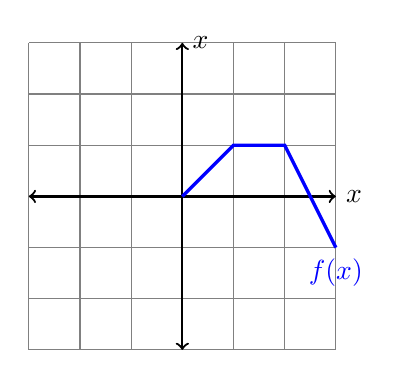
\begin{tikzpicture}[scale=0.65]
                    \draw[color=gray] (-3,-3) grid (3,3);
                    \draw[thick, black, <->] (-3,0) -- (3,0) node[anchor=west]{$x$};
                    \draw[thick, black, <->] (0,-3) -- (0,3) node[anchor=west]{$x$};
                    \draw[very thick, blue] (0,0) -- (1,1) -- (2,1) -- (3,-1)
                    node[anchor=north]{$f(x)$}; 
                \end{tikzpicture}
                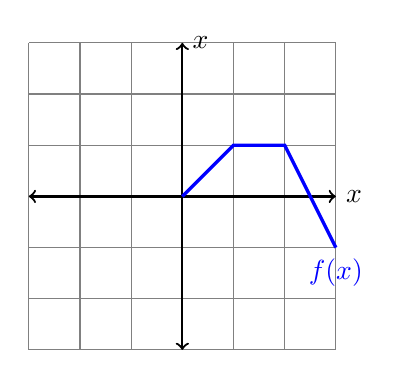
\begin{tikzpicture}[scale=0.65]
                    \draw[color=gray] (-3,-3) grid (3,3);
                    \draw[thick, black, <->] (-3,0) -- (3,0) node[anchor=west]{$x$};
                    \draw[thick, black, <->] (0,-3) -- (0,3) node[anchor=west]{$x$};
                    \draw[very thick, blue] (0,0) -- (1,1) -- (2,1) -- (3,-1)
                    node[anchor=north]{$f(x)$}; 
                \end{tikzpicture}
                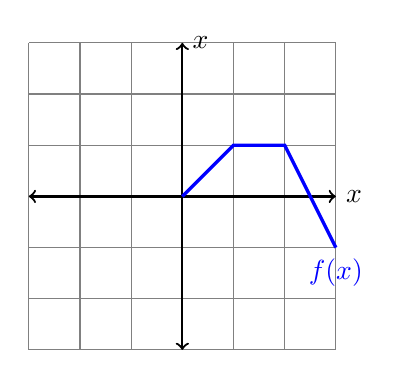
\begin{tikzpicture}[scale=0.65]
                    \draw[color=gray] (-3,-3) grid (3,3);
                    \draw[thick, black, <->] (-3,0) -- (3,0) node[anchor=west]{$x$};
                    \draw[thick, black, <->] (0,-3) -- (0,3) node[anchor=west]{$x$};
                    \draw[very thick, blue] (0,0) -- (1,1) -- (2,1) -- (3,-1)
                    node[anchor=north]{$f(x)$}; 
                \end{tikzpicture}
            \end{center}
    \ea
\end{activity}\aftera
